\textbf{Pregunta 3}
%\noindent
Describe una secuencia de accesos a un árbol splay $T$ de $n$ nodos, con $n \geq 5$ impar, que resulte en $T$
siendo una sola cadena de nodos en la que el camino para bajar en el árbol alterne entre hijo izquierdo e hijo derecho.
\newline

$\rhd$ \textbf{Solución:} Propongamos el siguiente árbol Splay\footnote{Su altura no es logarítmica,
pero sus consultas son amortizadas.}

\begin{center}
  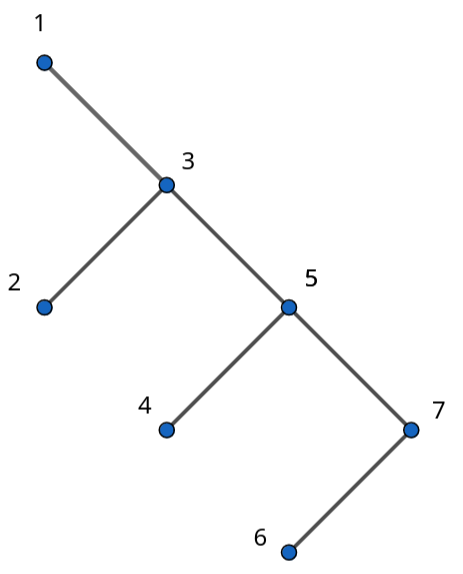
\includegraphics[scale=0.4]{./01.png}
\end{center}

Accedamos a $2$ realizando \code{Zig(2)} seguido de la operación \code{Zag(2)}:
\begin{center}
  \begin{figure}[h]
    \centering
    \subfloat[Zig(2)]{
      \label{f:02}
      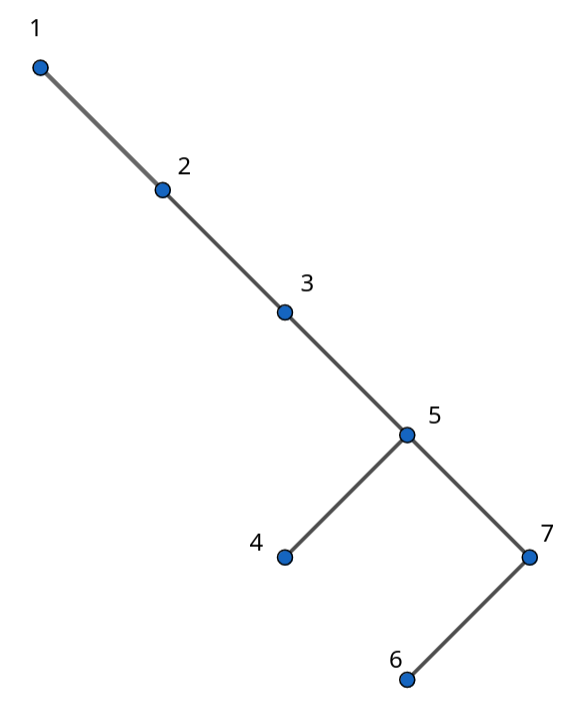
\includegraphics[width=0.4\textwidth]{02.png}}
    \subfloat[Zag(2)]{
      \label{f:03}
      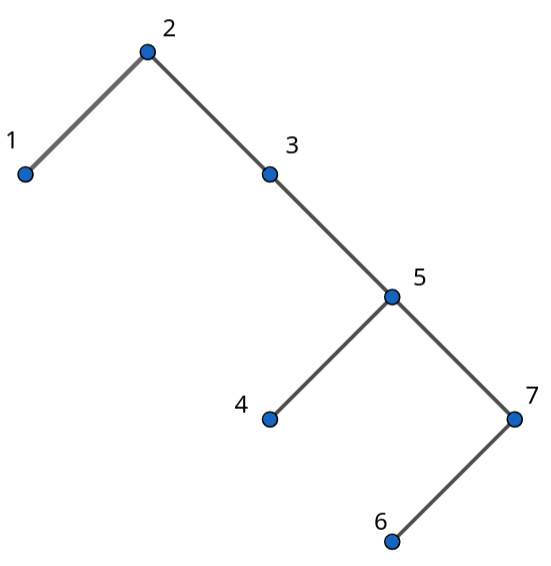
\includegraphics[width=0.4\textwidth]{03.png}}
    \caption*{Acceder a 2.}
    \label{f:animales}
  \end{figure}


  %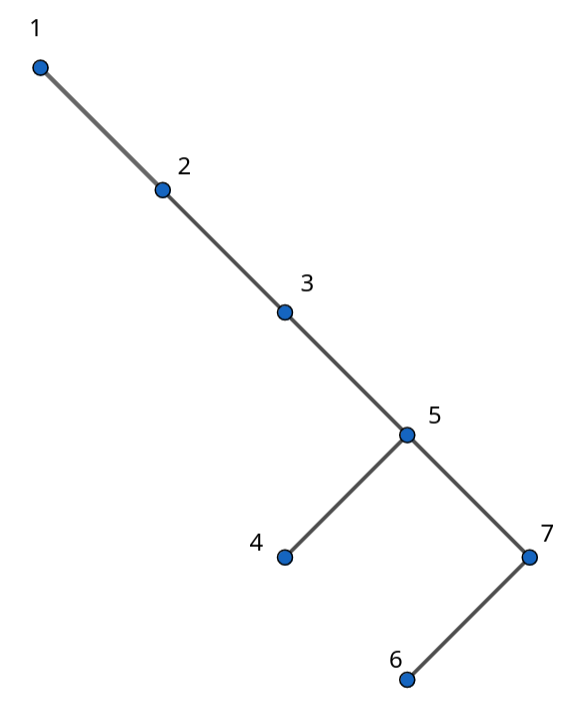
\includegraphics[scale=0.3]{./02.png}
\end{center}

Ahora, accedamos a $3$ realizando un \code{Zag(3)}

\begin{center}
  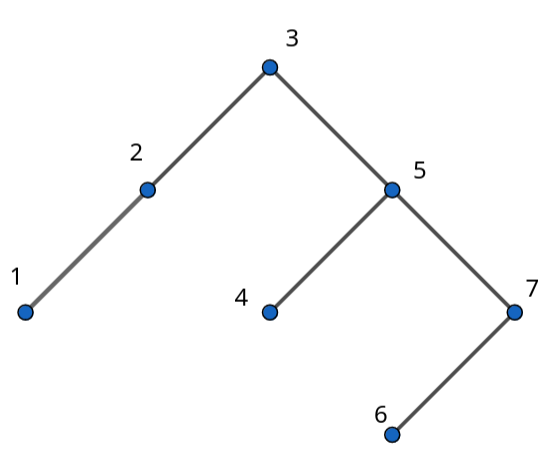
\includegraphics[scale=0.3]{./04.png}
\end{center}

Luego, accedamos a $4$ realizando \code{Zig(4)} seguido de la operación \code{Zag(4)}:

\begin{center}
  \begin{figure}[h]
    \centering
    \subfloat[Zig(4)]{
      \label{f:05}
      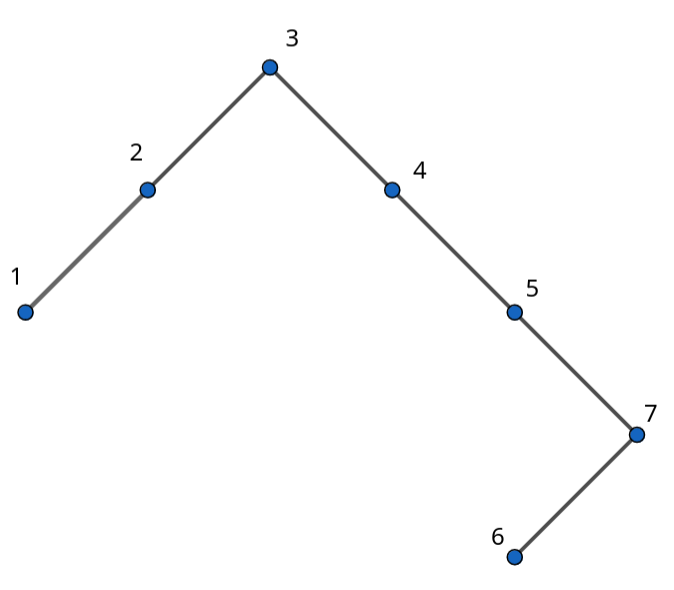
\includegraphics[width=0.4\textwidth]{05.png}}
    \subfloat[Zag(4)]{
      \label{f:06}
      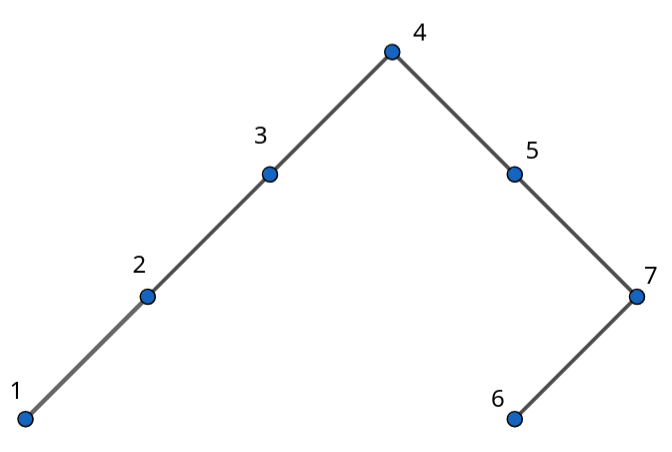
\includegraphics[width=0.4\textwidth]{06.png}}
    \caption*{Acceder a 4.}
    \label{f:animales}
  \end{figure}

  %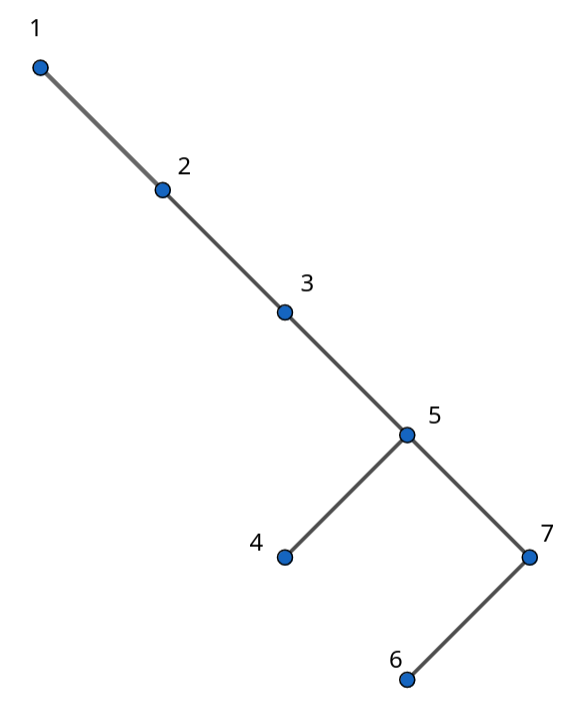
\includegraphics[scale=0.3]{./02.png}
\end{center}

Así, accedamos a $5$ realizando un \code{Zag(5)}

\begin{center}
  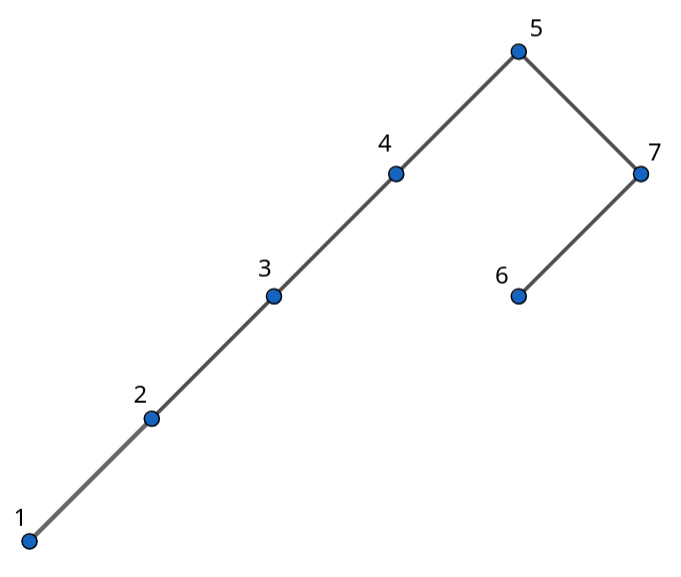
\includegraphics[scale=0.3]{./07.png}
\end{center}

\newpage
Luego, accedamos a $6$ realizando \code{Zig(6)} seguido de la operación \code{Zag(6)}:

\begin{center}
  \begin{figure}[h]
    \centering
    \subfloat[Zig(6)]{
      \label{f:08}
      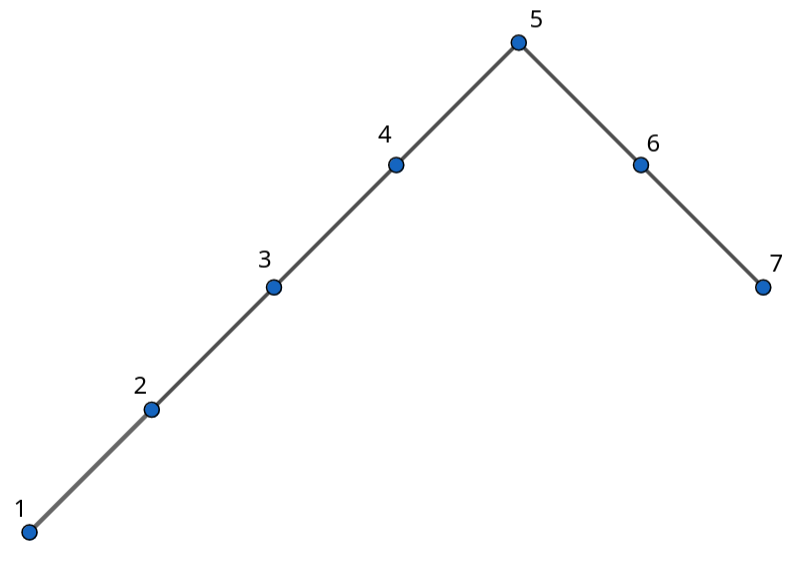
\includegraphics[width=0.4\textwidth]{08.png}}
    \subfloat[Zag(6)]{
      \label{f:09}
      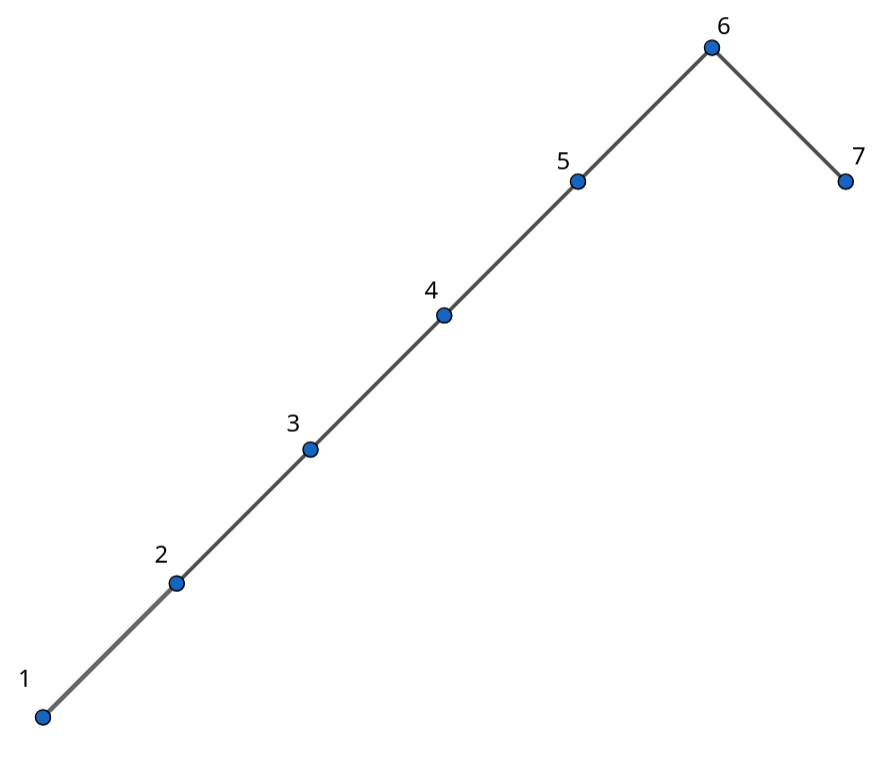
\includegraphics[width=0.4\textwidth]{09.png}}
    \caption*{Acceder a 6.}
    \label{f:animales}
  \end{figure}

  %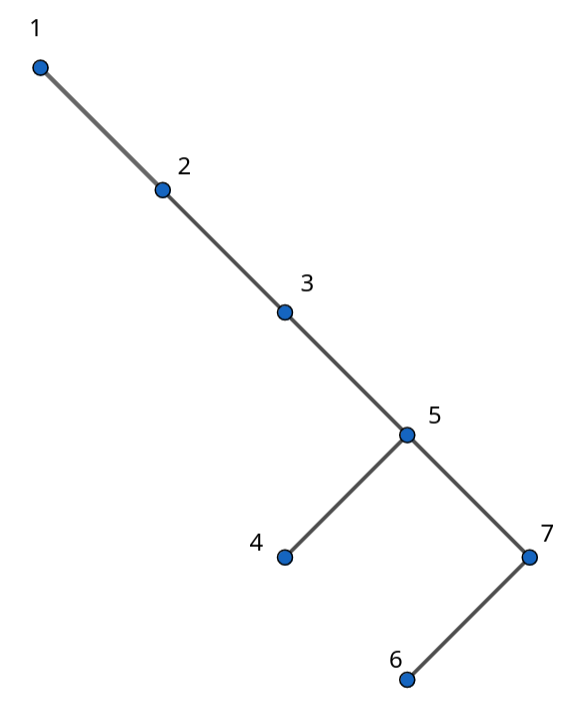
\includegraphics[scale=0.3]{./02.png}
\end{center}

Por último, accedamos a $7$ realizando un \code{Zag(7)}

\begin{center}
  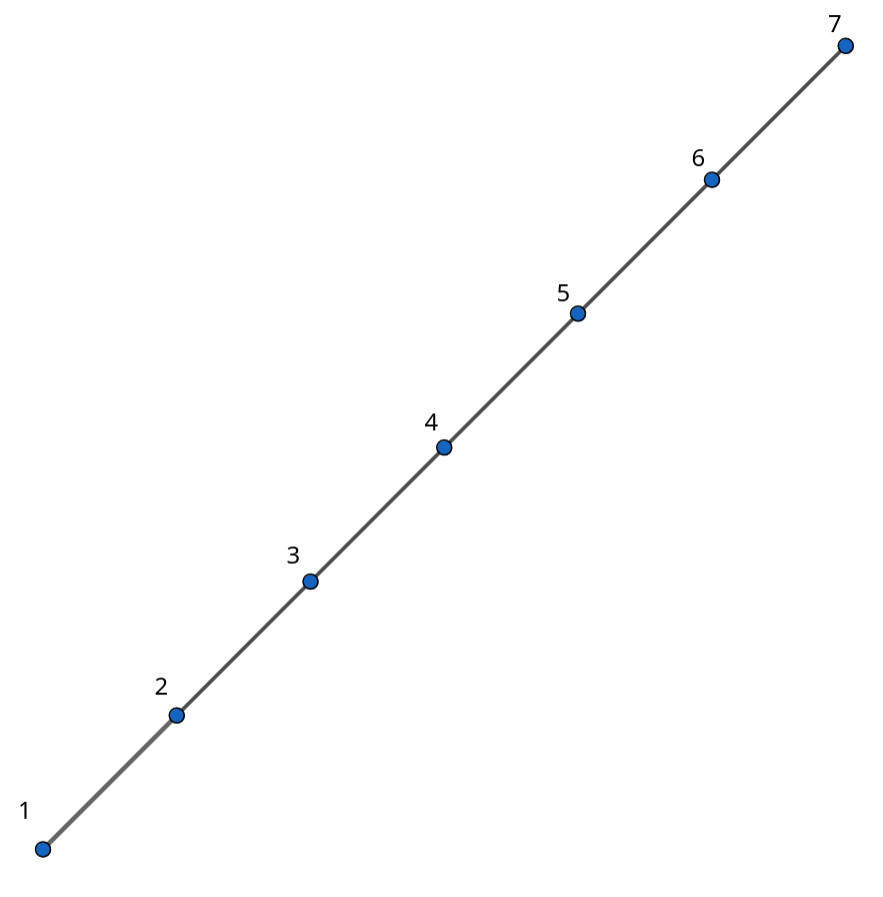
\includegraphics[scale=0.3]{./10.png}
\end{center}

Cómo podemos notar; $7 \rightarrow$ derecho, $6 \rightarrow$ izquierdo, $5 \rightarrow$ derecho,
$4 \rightarrow$ izquierdo, $3 \rightarrow$ derecho, $2 \rightarrow$ izquierdo, y por último tenemos
al $1$ que en primer instancia fue la raíz y por vacuidad podemos asumir que es un hijo derecho.\newline

De lo anterior, hemos encontrado una cadena de nodos tal que al decender por la raíz hasta la hoja se encuentran
los elementos iniciales de manera alternada entre hijos izquierdos y derechos.
\hfill $\lhd$
%\subsection*{Respuesta}

%<Tu respuesta aquí>

%\bigskip
